\documentclass{beamer}
\usetheme{default}
\usecolortheme{beaver}
\usepackage{graphicx}
\usepackage{hyperref}
\usepackage{tikz}
\usepackage[final]{pdfpages}
\usetikzlibrary{positioning}
%\usetikzlibrary{arrows}
%\useinnertheme{circles}
\setbeamercolor{itemize item}{fg=black}
\setbeamercolor{itemize subitem}{fg=darkred}
\setbeamercolor{itemize subsubitem}{fg=black}
\setbeamercolor{title}{fg=darkred, bg=white}

%\setbeamercolor{enumerate items}{darkred, white}
\setbeamercolor{block body}{bg=gray!10, fg=black}
\setbeamercolor{button}{bg=darkred,fg=white}
%\setbeamercolor{block title}{bg=red!20, fg=black}
%\settowidth{\leftmargini}{\usebeamertemplate{itemize item}}
%\addtolength{\leftmargini}{\labelsep}
%\setlength{\leftmargini}{0pt}
\setbeamertemplate{navigation symbols}{}

\title{The Effect of Streaming Chat \\ on Perceptions of Debates
}
\subtitle{}
\author{Victoria Asbury (Harvard)\\ Keng-Chi Chang (UCSD)\\ Katherine McCabe (Rutgers) \\
Kevin Munger (Penn State)\\ Tiago Ventura (U of Maryland)\footnote{This research is supported by a grant from the Russell Sage Foundation through the Summer Institute in Computational Social Science.}}
\date{\today}
\institute{FGV-DAPP}


\begin{document}

\begin{frame}
\titlepage
\end{frame}

\begin{frame}
\frametitle{Summary}


We conduct a ``field" experiment that assigns would-be debate viewers to watch the October 2019 Dem Debate

\pause 
\vspace{3mm}
\begin{itemize}
    \item Three contexts \pause 
    \begin{itemize}
        \item Control (standard NBC broadcast)
        \item Expert chat (538 website)
        \item Streaming chat (Facebook)
    \end{itemize}

\end{itemize}
\end{frame}


\begin{frame}
\frametitle{Rise of Streaming Chat}

\centering
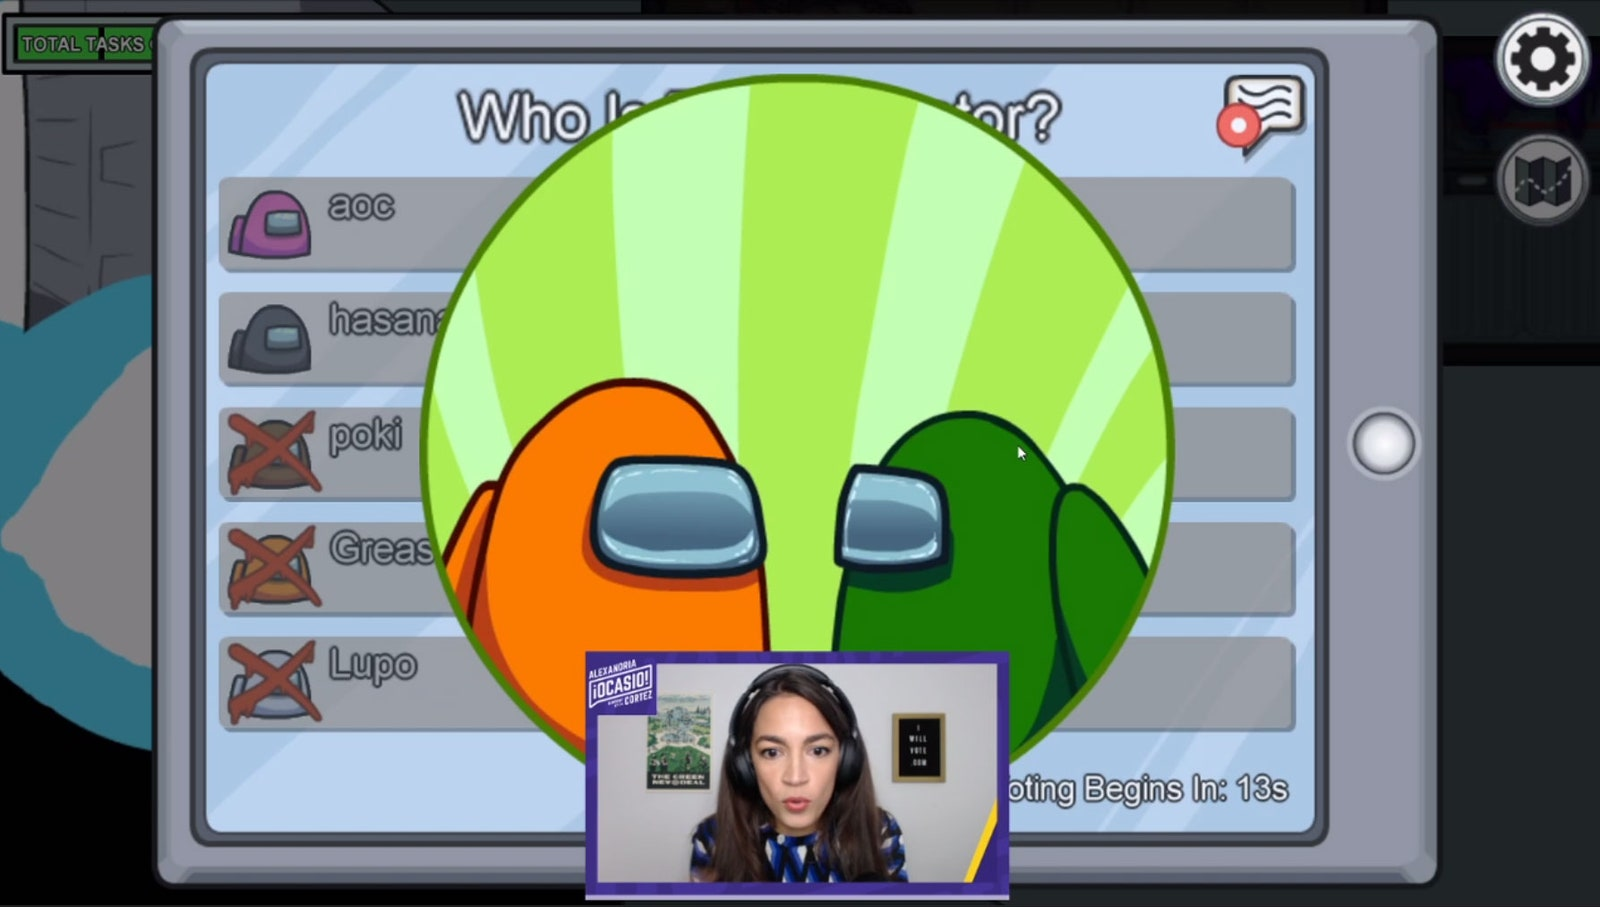
\includegraphics[width=.4\linewidth]{aoc2.jpg}\\
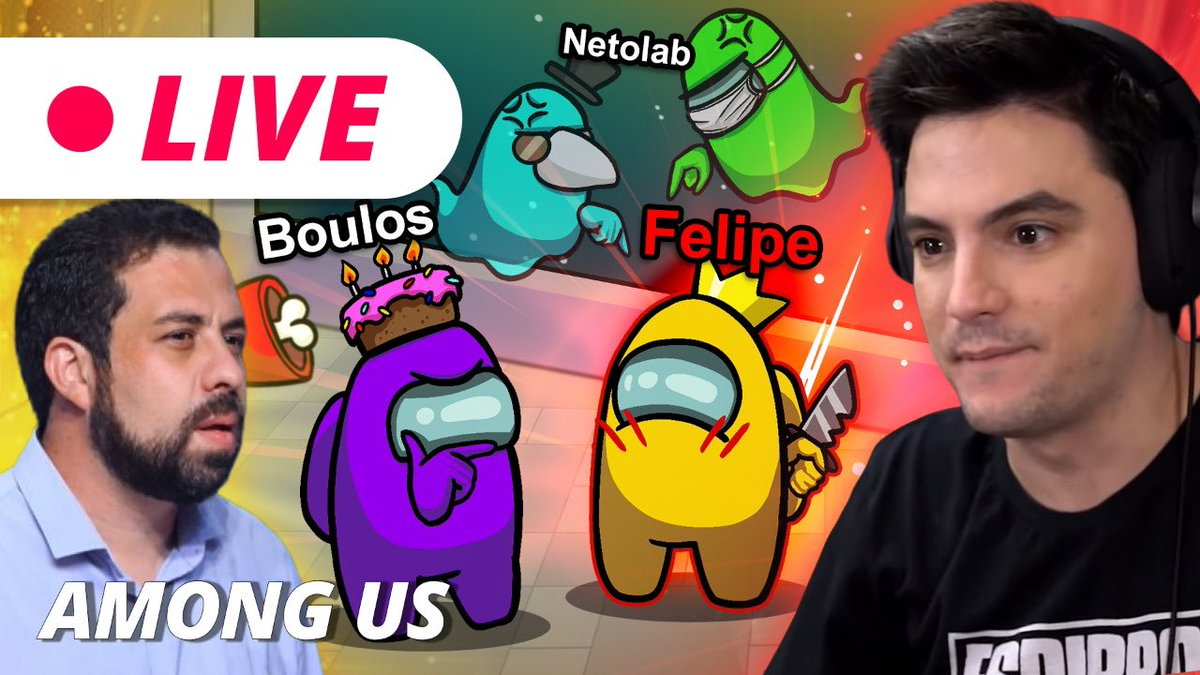
\includegraphics[width=.4\linewidth]{boulos.jpg}

\includegraphics[width=.35\linewidth]{istoe.jpg}\\

\end{frame}


\begin{frame}
\frametitle{Streaming Chat: Characteristics and Definitions}

\pause 
\vspace{3mm}
\begin{itemize}
    \item Streaming Chats + Video Feed + All in one screen. \pause
    \item Most of times: chaotic conversations. \pause 
    \item Popular among the young \pause 
    \begin{itemize}
        \item Twitch (Amazon)
        \item YouTube/YouTube Gaming (Google)
        \item Mixer (Microsoft)
    \end{itemize}
    \pause 
\end{itemize}



\end{frame}



\begin{frame}
\frametitle{Related Literature: Dual Screening}


Dual Screen: Users engage real-time conversations on a second screen (Twitter). 

\pause

\vspace{3mm}
\begin{itemize}
    \item Initial concern about ``distraction" supplanted by thinking about purposiveness ( (Gottfried et al., 2017; Van Cauwenberge et al.,
2015, 2014)
      \begin{itemize}
        \item Viewers decide how to allocate their attention  (McGregor
and Mourão, 2017
    \end{itemize}
\end{itemize}

\begin{itemize}
    \item Changes the emphasis on what is observed: \textit{priming}  (Barnidge et al., 2017)
\end{itemize}  
\begin{itemize}
    \item Changes in Political Behavior and Attitudes
    \begin{itemize}
        \item Dual Screening generates more online political engagement (Barnidge et al., 2017; Gil de
Zúñiga et al., 2015; McGregor and Mourão, 2017; Vaccari et al., 2015
    \end{itemize}
\end{itemize}
\end{frame}





\begin{frame}
\frametitle{New Features of Streaming Chats}
\pause 
\vspace{3mm}
\begin{itemize}
\item Streaming chat: different audience, different technology
    \pause 
      \begin{itemize}
       % \item Who is watching the Facebook livestream of a debate? \pause
        \item Chat streams at eye-level; only one conversation (no personalization/viewer discretion)
        \item Thousands of comments, difficult to follow, and one only observes nodes of the network (majority illusion). 
        \item More cross-cutting information
        \pause 
    \end{itemize}
        \vspace{3mm}
        \pause
\item Shift from genteel (possibly partisan) broadcasters towards the garbage fire that is comment sections
    \pause 
      \begin{itemize}
        \item No moderation in real-time \pause
        \item Lots of repetition/``memes"  \pause 
\end{itemize}
        \pause

        \vspace{3mm}
    \item Priming a very different set of issues
      \begin{itemize}
       % \item Many are outside the scope of standard politics \pause
        \item Maybe good (elite primes downplay serious attacks on candidate weakness)
        \item Maybe bad (reinforcing anti-deliberative, discriminatory and even hateful primes)
    \end{itemize}
        \pause 

\end{itemize}

\end{frame}









\begin{frame}
\frametitle{Summary of Theoretical Pathways}

How does streaming chat influence perceptions of political events?

\begin{itemize}
    \item \textbf{Frequency}: High volume comments increases distraction and information overload. 
    \item \textbf{Content}: Topics discussed serve as primes.
    \item \textbf{Context}: Commenter composition leads to inaccurate inferences of overall public opinion (danger for toxic speech).
\end{itemize}

\end{frame}


\begin{frame}
\frametitle{Research Design and Sample}

Facebook (Social) vs. ABC (Control) vs. FiveThirtyEight (Expert)

\centering
\includegraphics[width=.4\linewidth]{screenshot-fbblurcopy.png}\\
\includegraphics[width=.4\linewidth]{screenshot-abc.png}
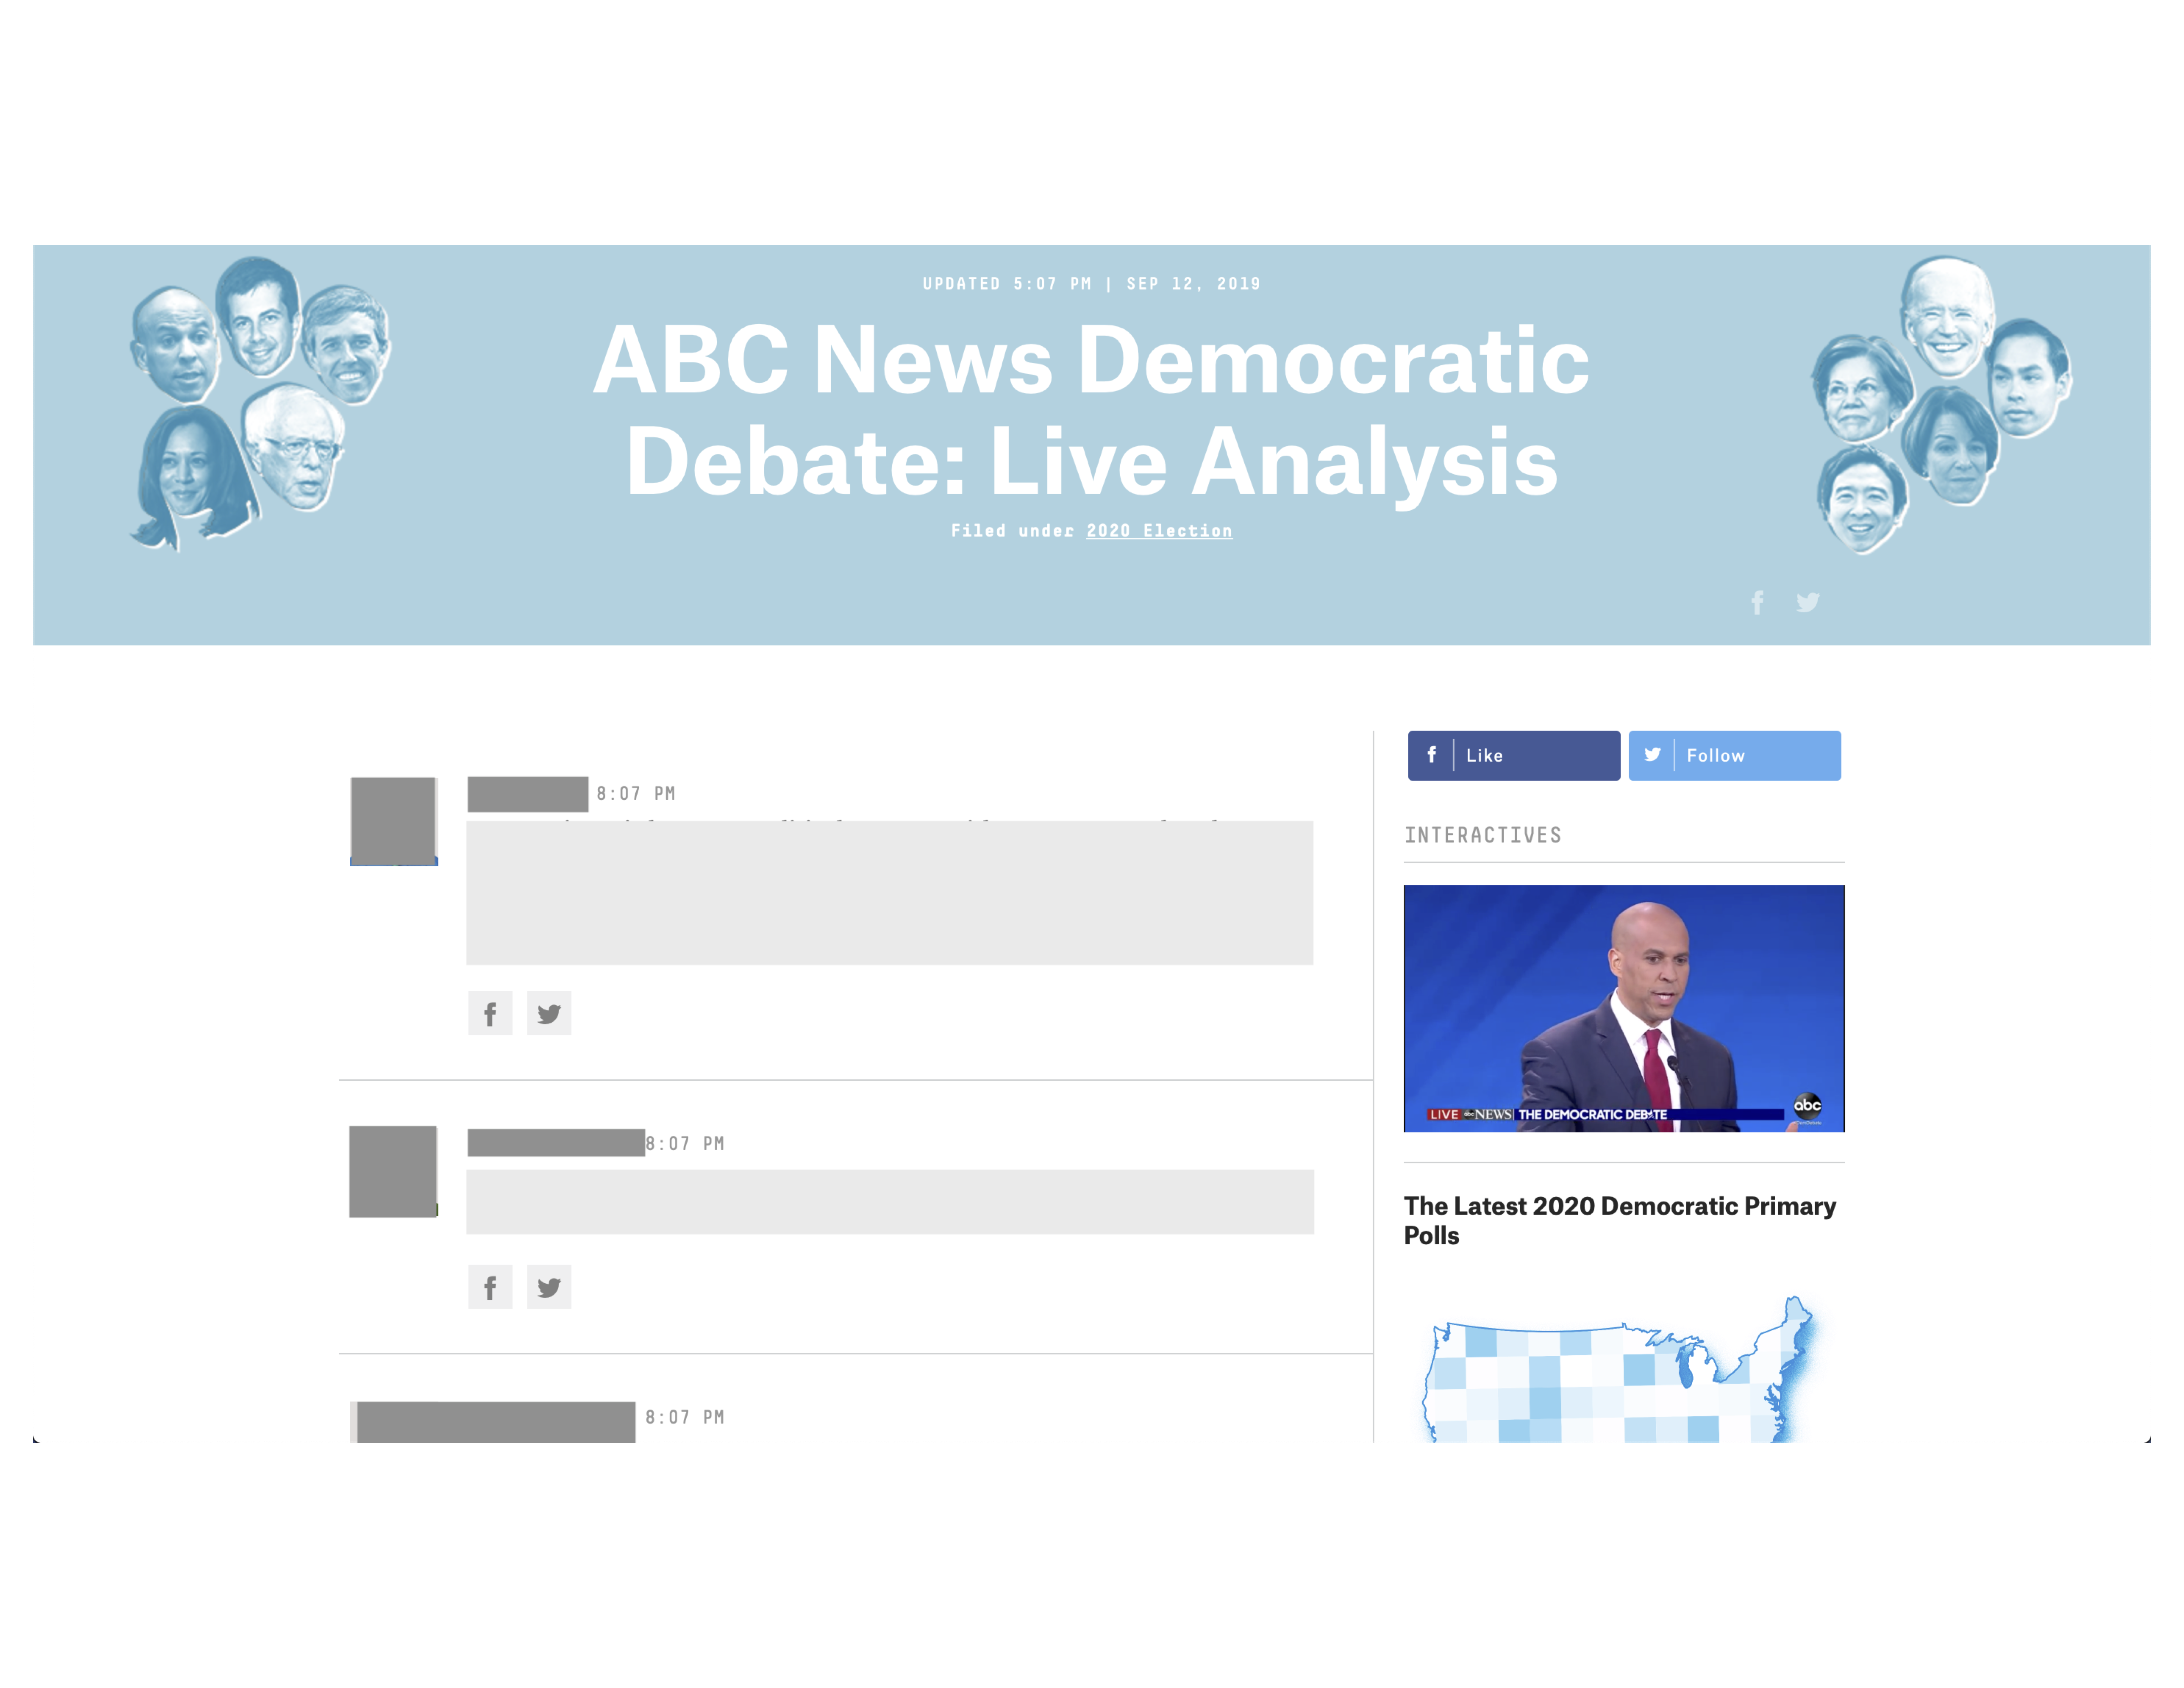
\includegraphics[width=.35\linewidth]{screenshot-538-blurcopy.png}\\

\end{frame}


\begin{frame}
\frametitle{Research Design and Sample}

Two-Wave Survey September 2019 through MTurk (following Gross, Porter and Wood, 2019). 

\vspace{3mm}
\begin{itemize}
    \item Wave 1 pre-debate survey with 2352 respondents
    \begin{itemize}
        \item Identified respondents likely to watch debate, have Facebook account, could watch debate on a computer.
    \end{itemize}
    
    \vspace{3mm}
    \item Encouraged 1095 eligible and interested participants to watch debate on randomly assigned platform.
    
    \vspace{3mm}
    \item Wave 2 survey with 908 respondents
      \begin{itemize}
        \item Analysis focuses on 576 Wave 2 Democratic respondents (including leaners) who watched at least part of the debate
        \item N= 204 (Control), N= 174 (Expert), N= 198 (Social)
    \end{itemize}
\end{itemize}

\vspace{3mm}
Extract and analyze comments from Facebook and FiveThirtyEight streaming chat.

\end{frame}


\begin{frame}
\frametitle{Hypotheses}

\scriptsize
\begin{table}
\begin{center}
\begin{tabular}{l p{35mm} p{38mm}  }
\hline


 & Social & Expert  \\
\hline
Frequency & (H1) Less enjoyable, informative, but more engaging & (H1e) More enjoyable, informative, engaging  \\ 

& (H2) More anxious and angry & (H2e) Less anxious and angry \\ \hline

Content & (H3) Comments increase in name recognition & (H3e) Comments increase in name recognition \\

& (H4) Prominent negative primes decrease candidate evaluations & 
(H4e) Prominent negative primes decrease candidate evaluations \\ \hline

Context & (H5) Decrease trust & (H5e) Increase trust \\ 
& (H6) Increase affective polarization & (H6e) Decrease affective polarization \\
& (H7) Positive comments increase perception of future performance  & (H7e) No change in perception of future performance \\ \hline


\end{tabular}
\end{center}
\end{table}


\end{frame}



\begin{frame}
\frametitle{Text Analysis: Validating Theoretical Premises}
\centering

Social Media Comments are very frequent
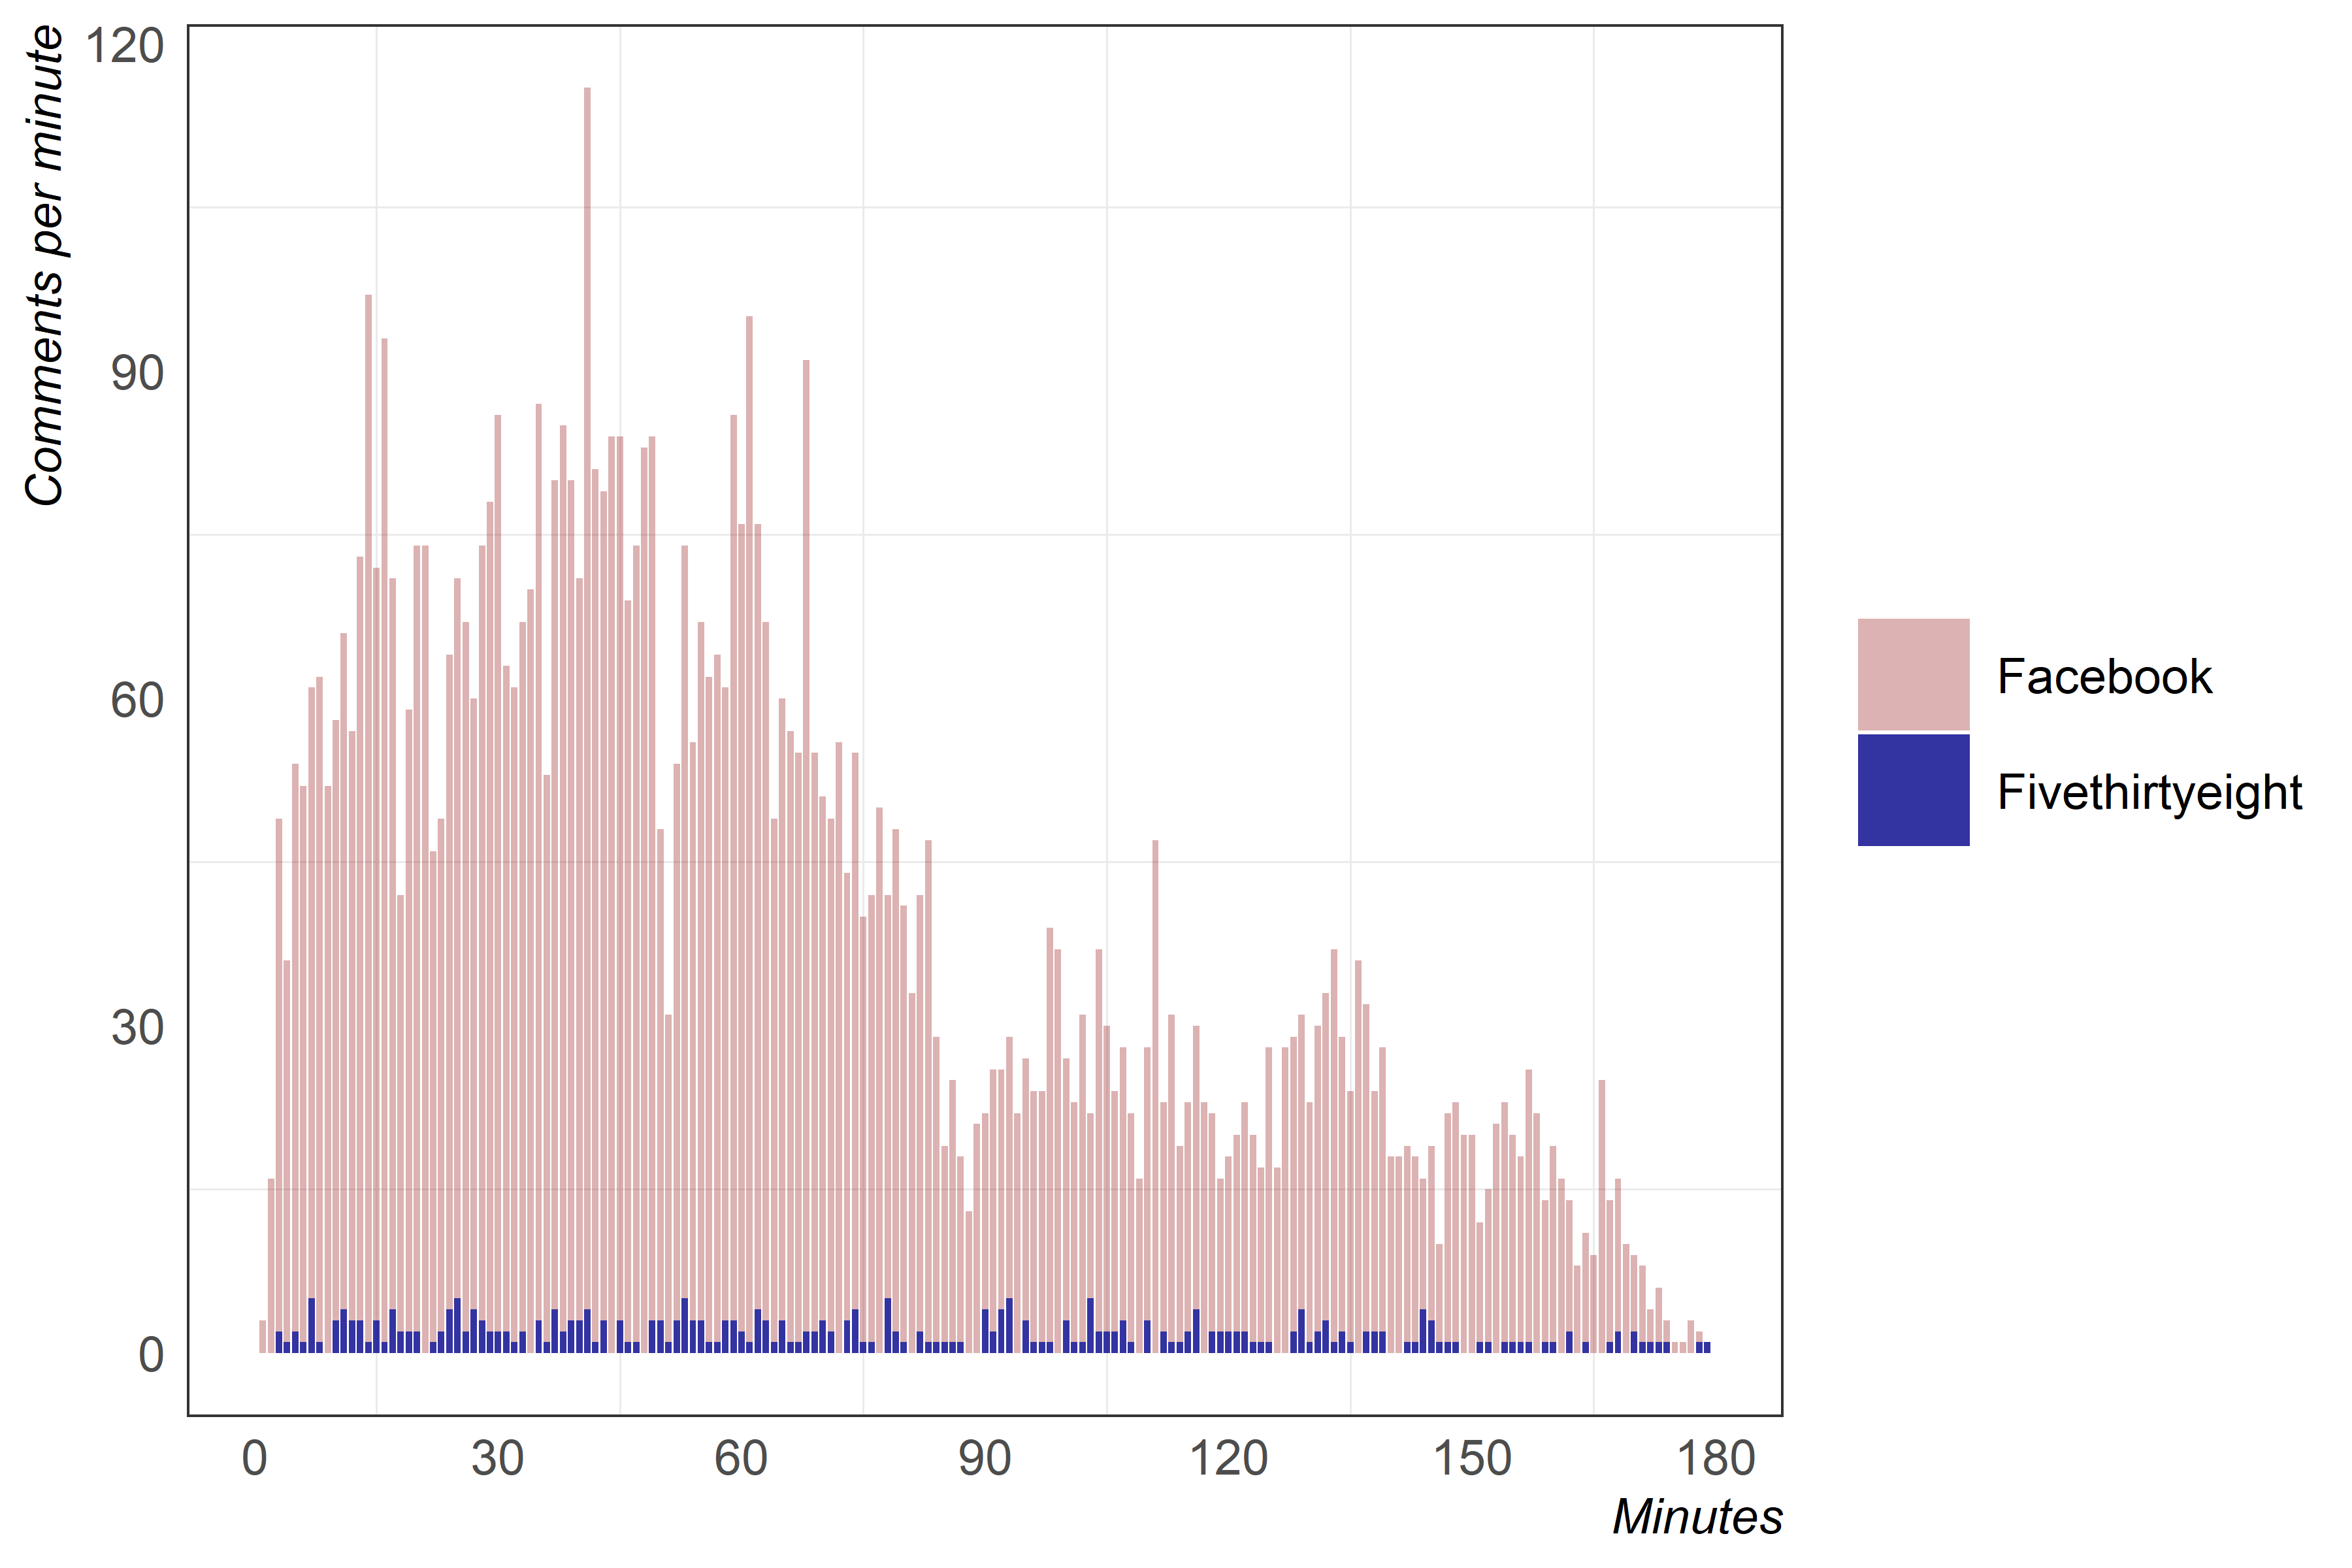
\includegraphics[width=1\linewidth]{freq-bind.png}

\end{frame}


\begin{frame}
\frametitle{Text Analysis: Validating Theoretical Premises}
\centering

Much more toxic

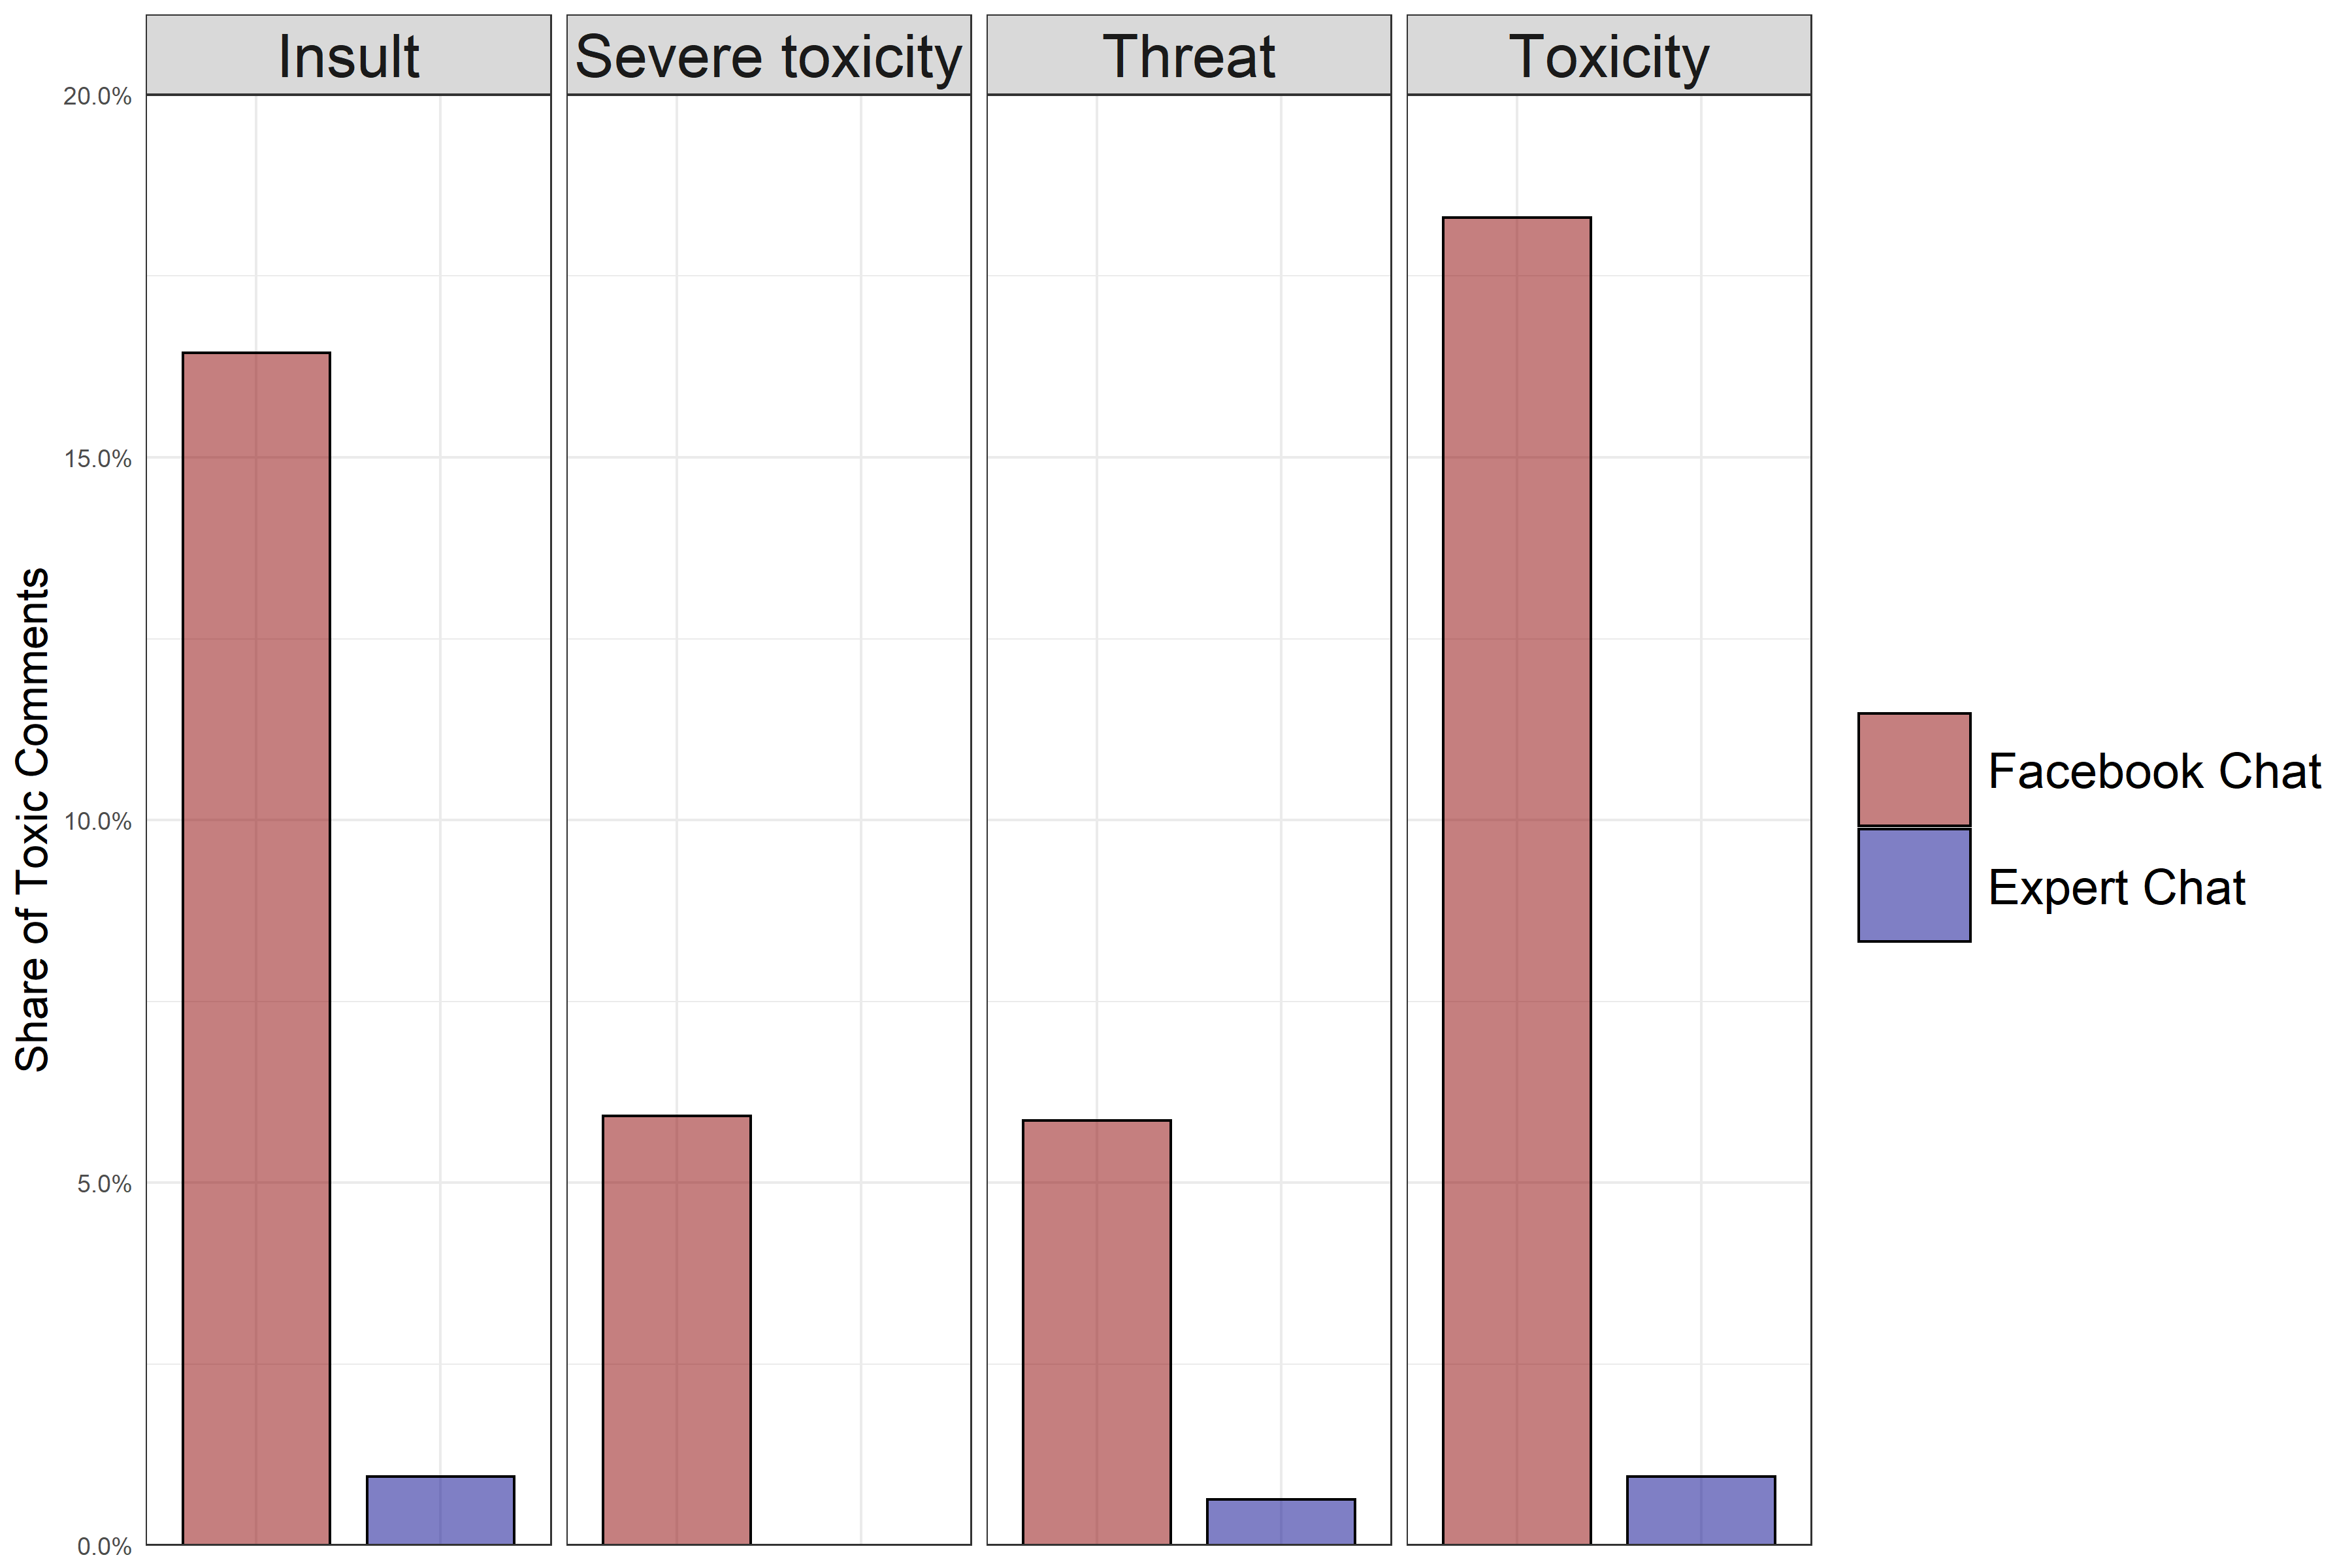
\includegraphics[width=1\linewidth]{proportion_toxicity.png}

\end{frame}



\begin{frame}
\frametitle{Text Analysis: Validating Theoretical Premises}
And contain prominent negative primes.
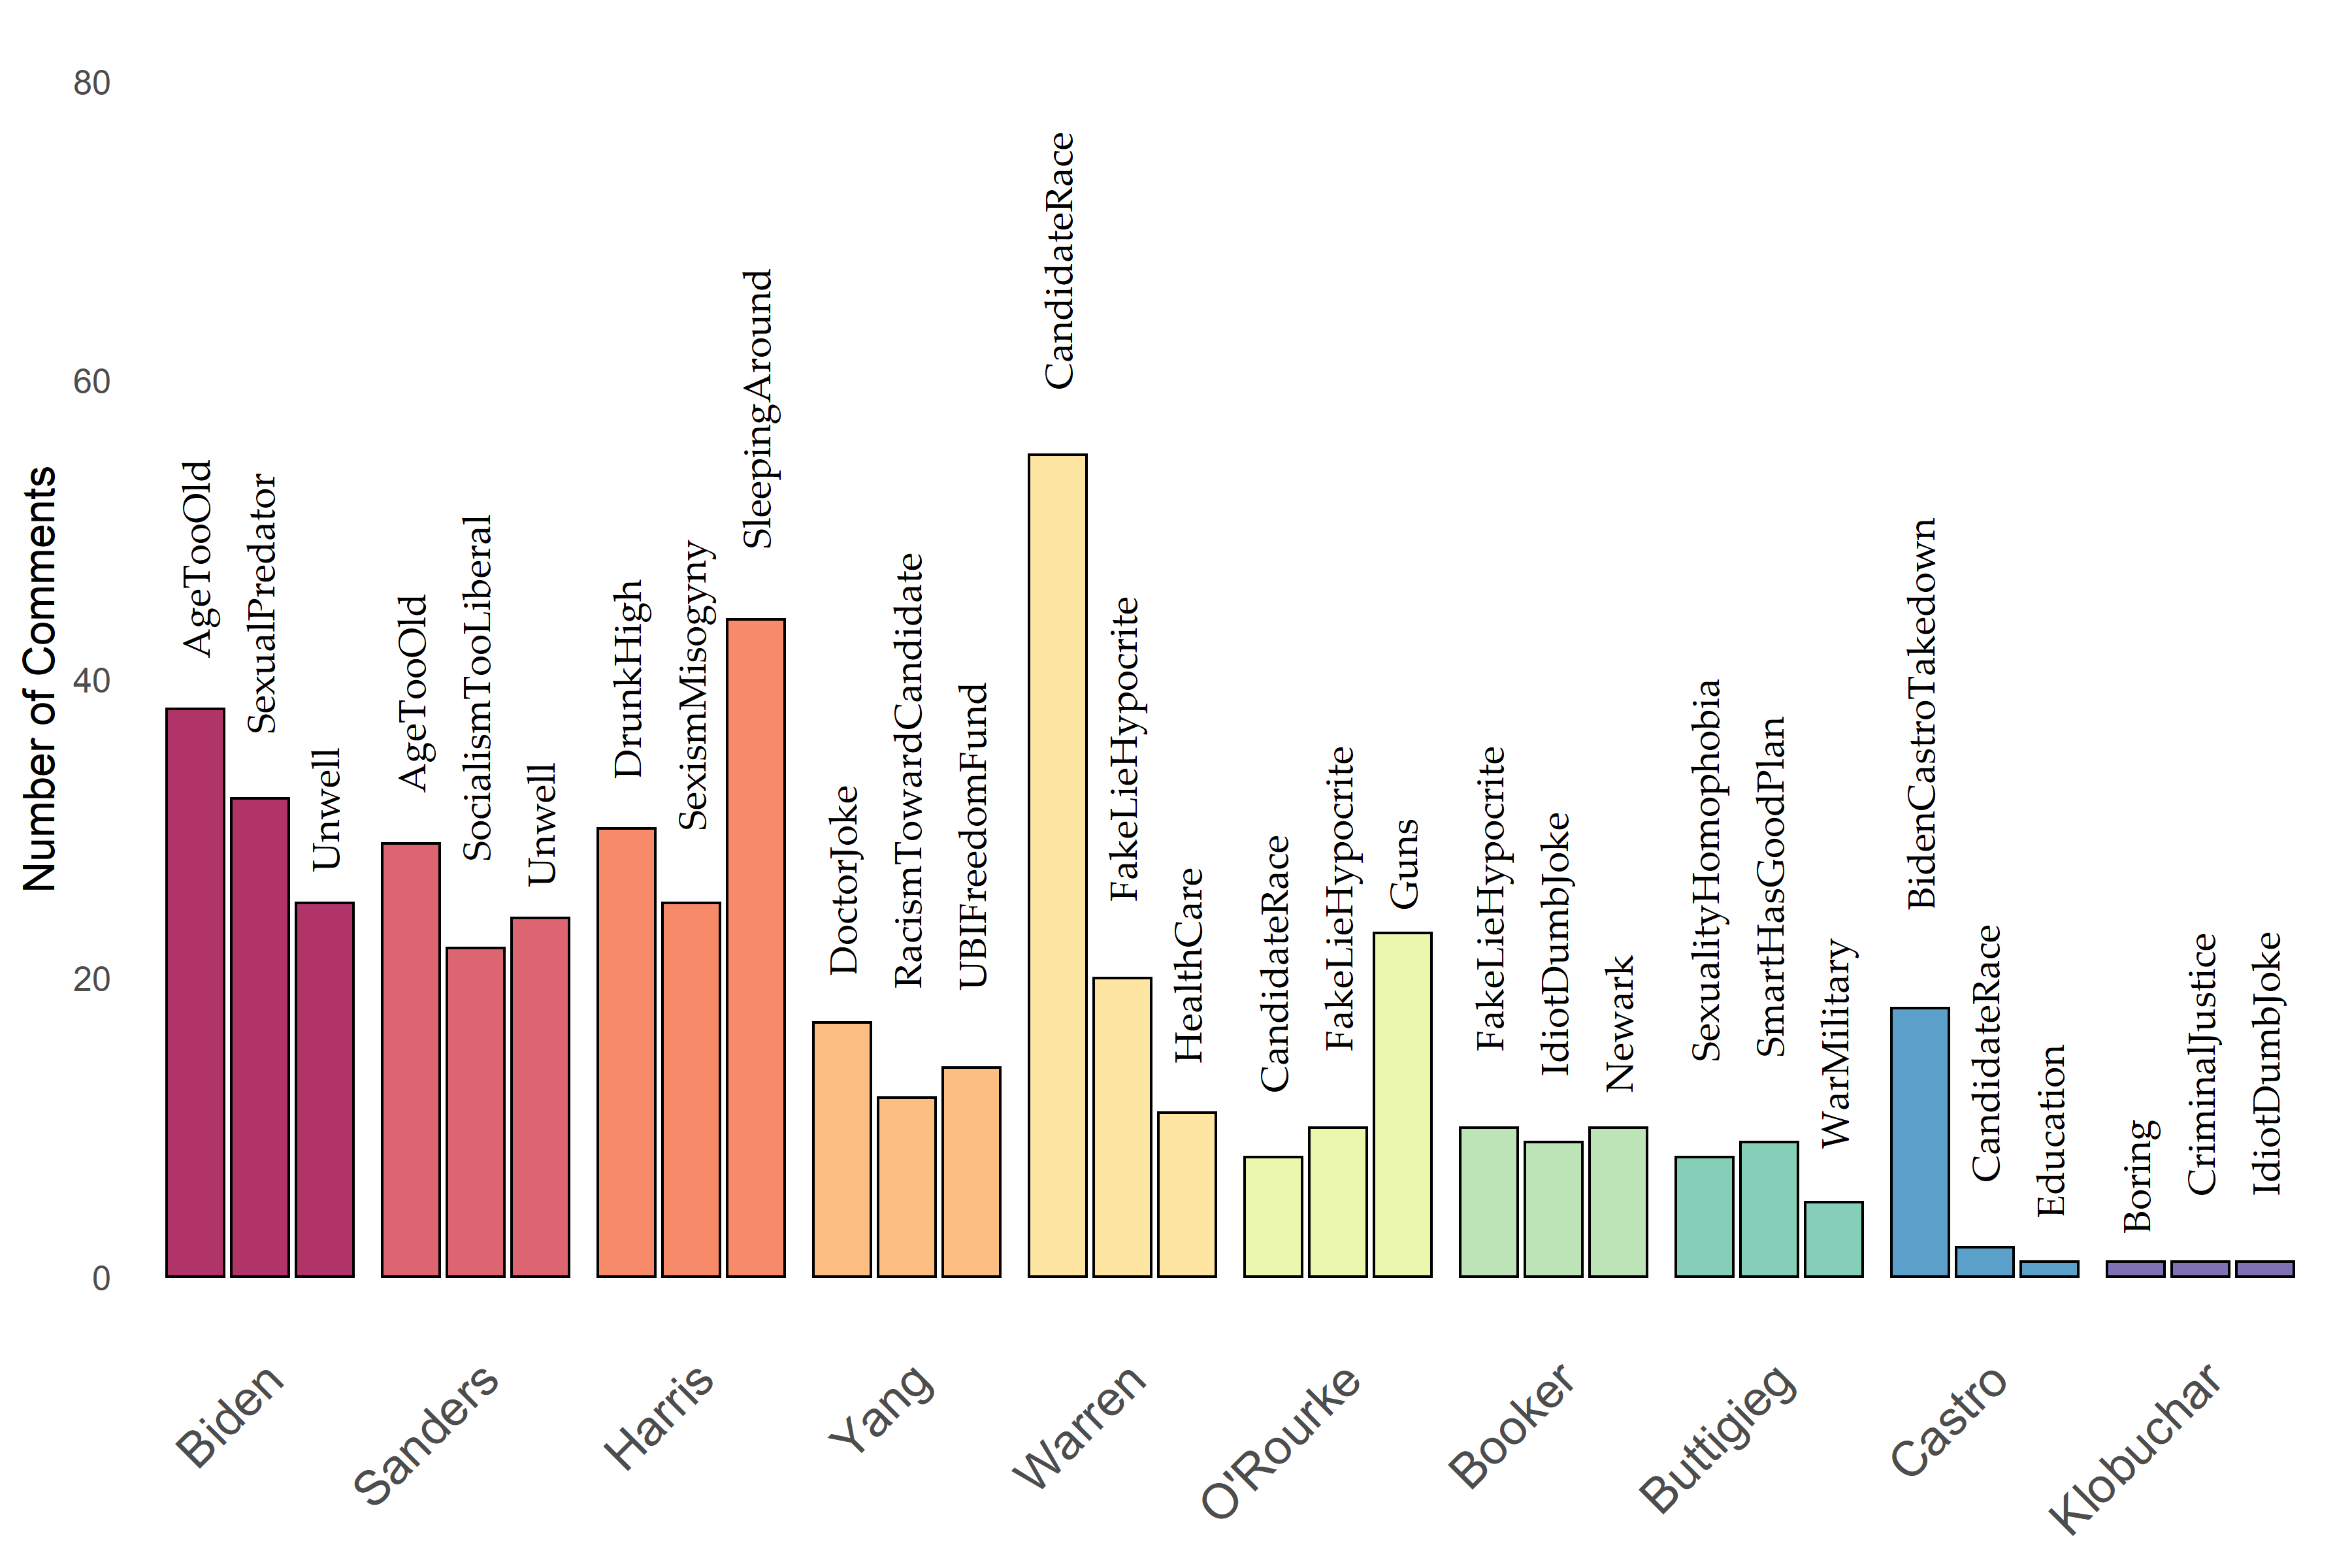
\includegraphics[width=1\linewidth]{topics_3by_cand.png}
\end{frame}


\begin{frame}
\frametitle{Frequency Hypothesis Key Results}

Social chat somewhat less informative, enjoyable, and engaging.

\centering
	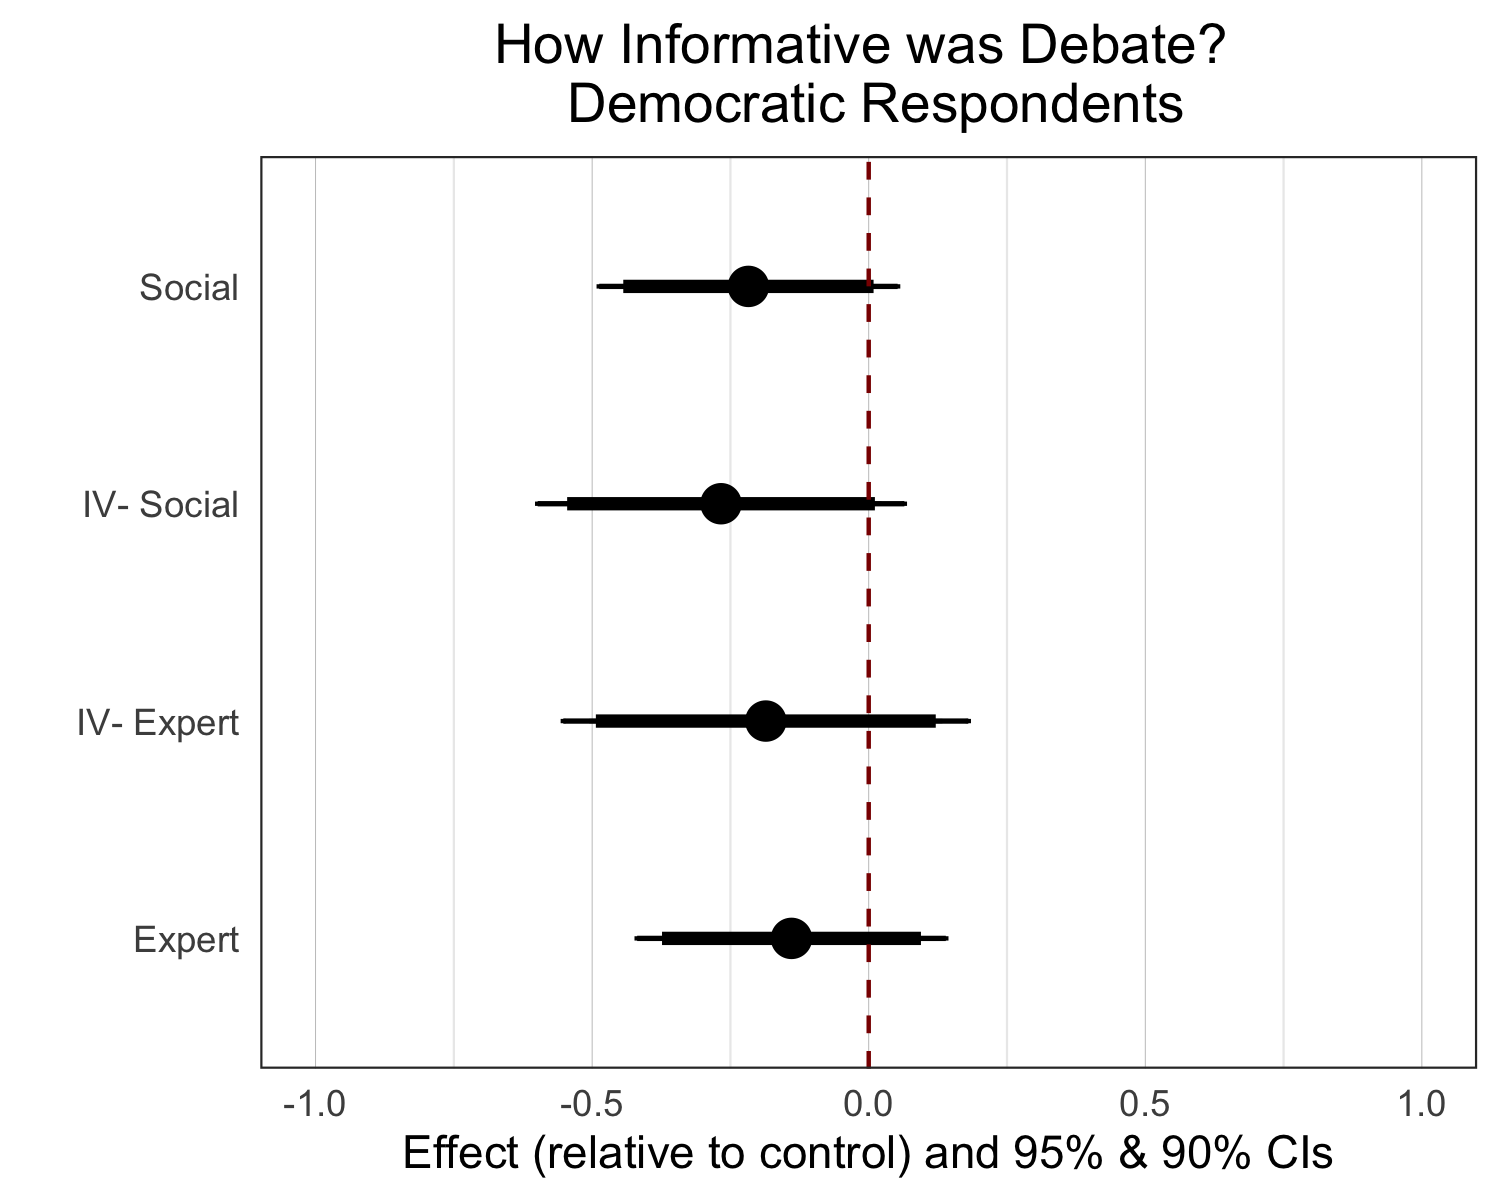
\includegraphics[width=.8\linewidth]{informative_dem.png}

\end{frame}

\begin{frame}
\frametitle{Frequency Hypothesis Key Results}

Social chat somewhat less informative, enjoyable, and engaging.

\centering
	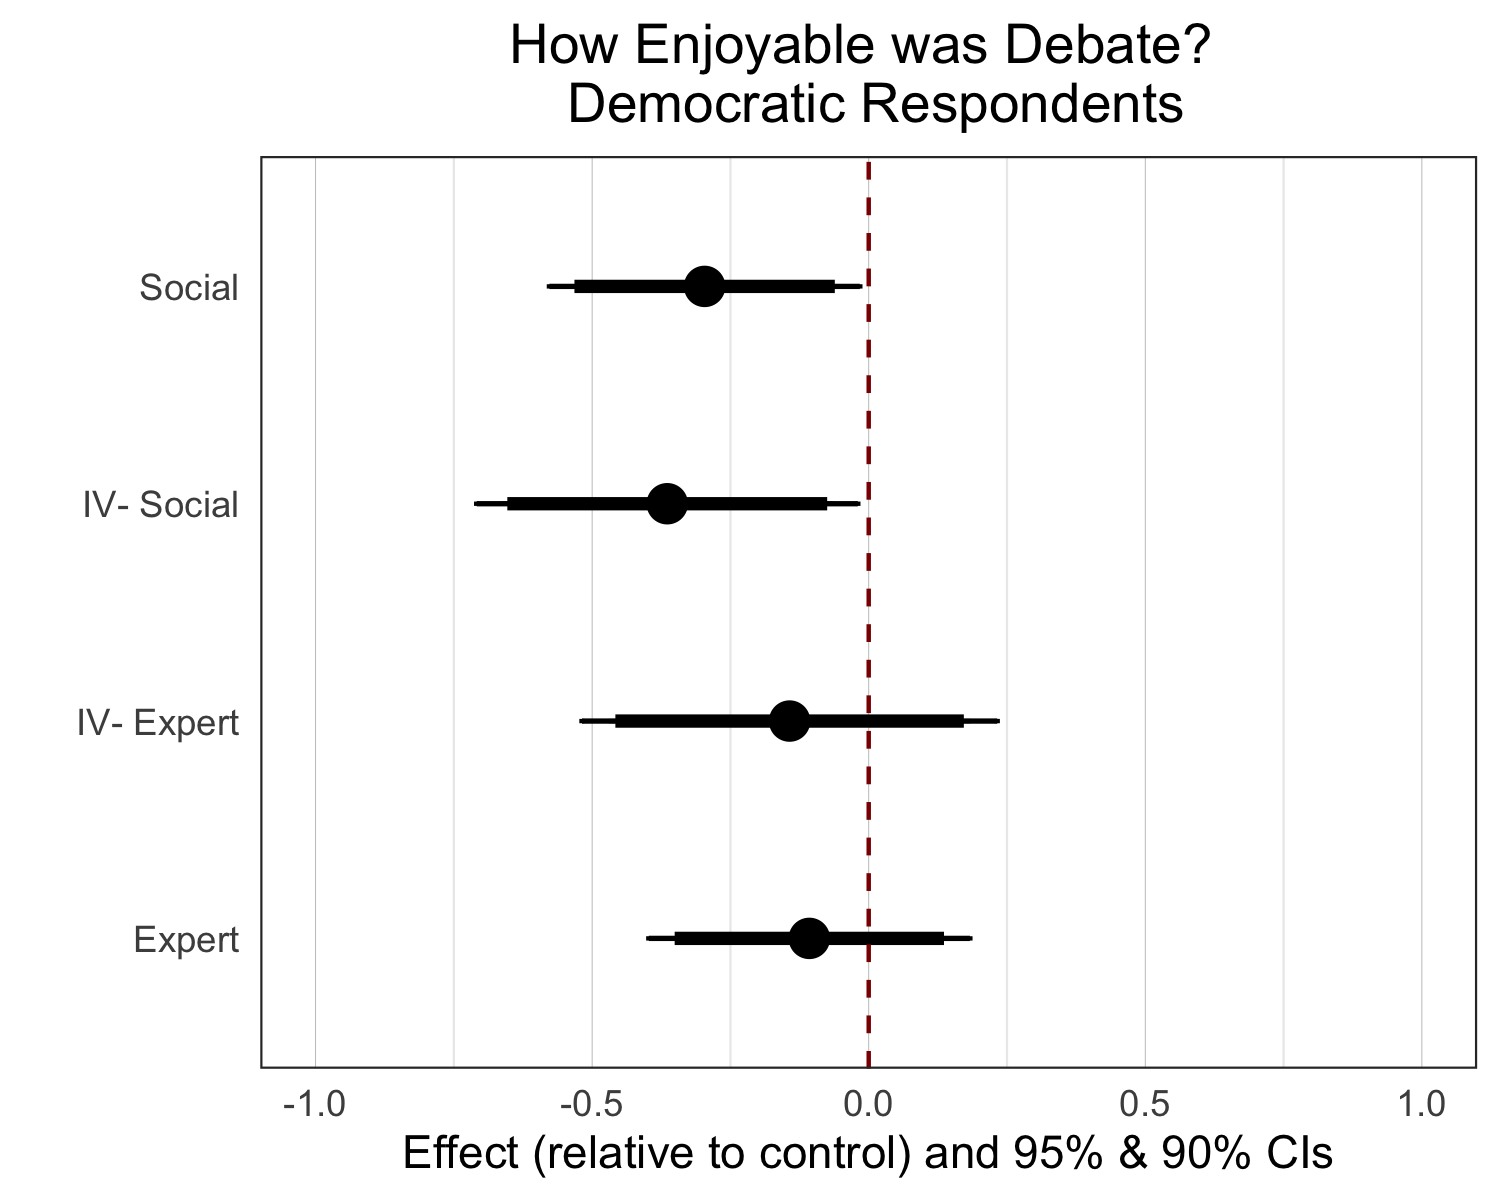
\includegraphics[width=.8\linewidth]{enjoyment_dem.png}\\

\end{frame}

\begin{frame}
\frametitle{Frequency Hypothesis Key Results}

Social chat somewhat less informative, enjoyable, and engaging.

\centering
	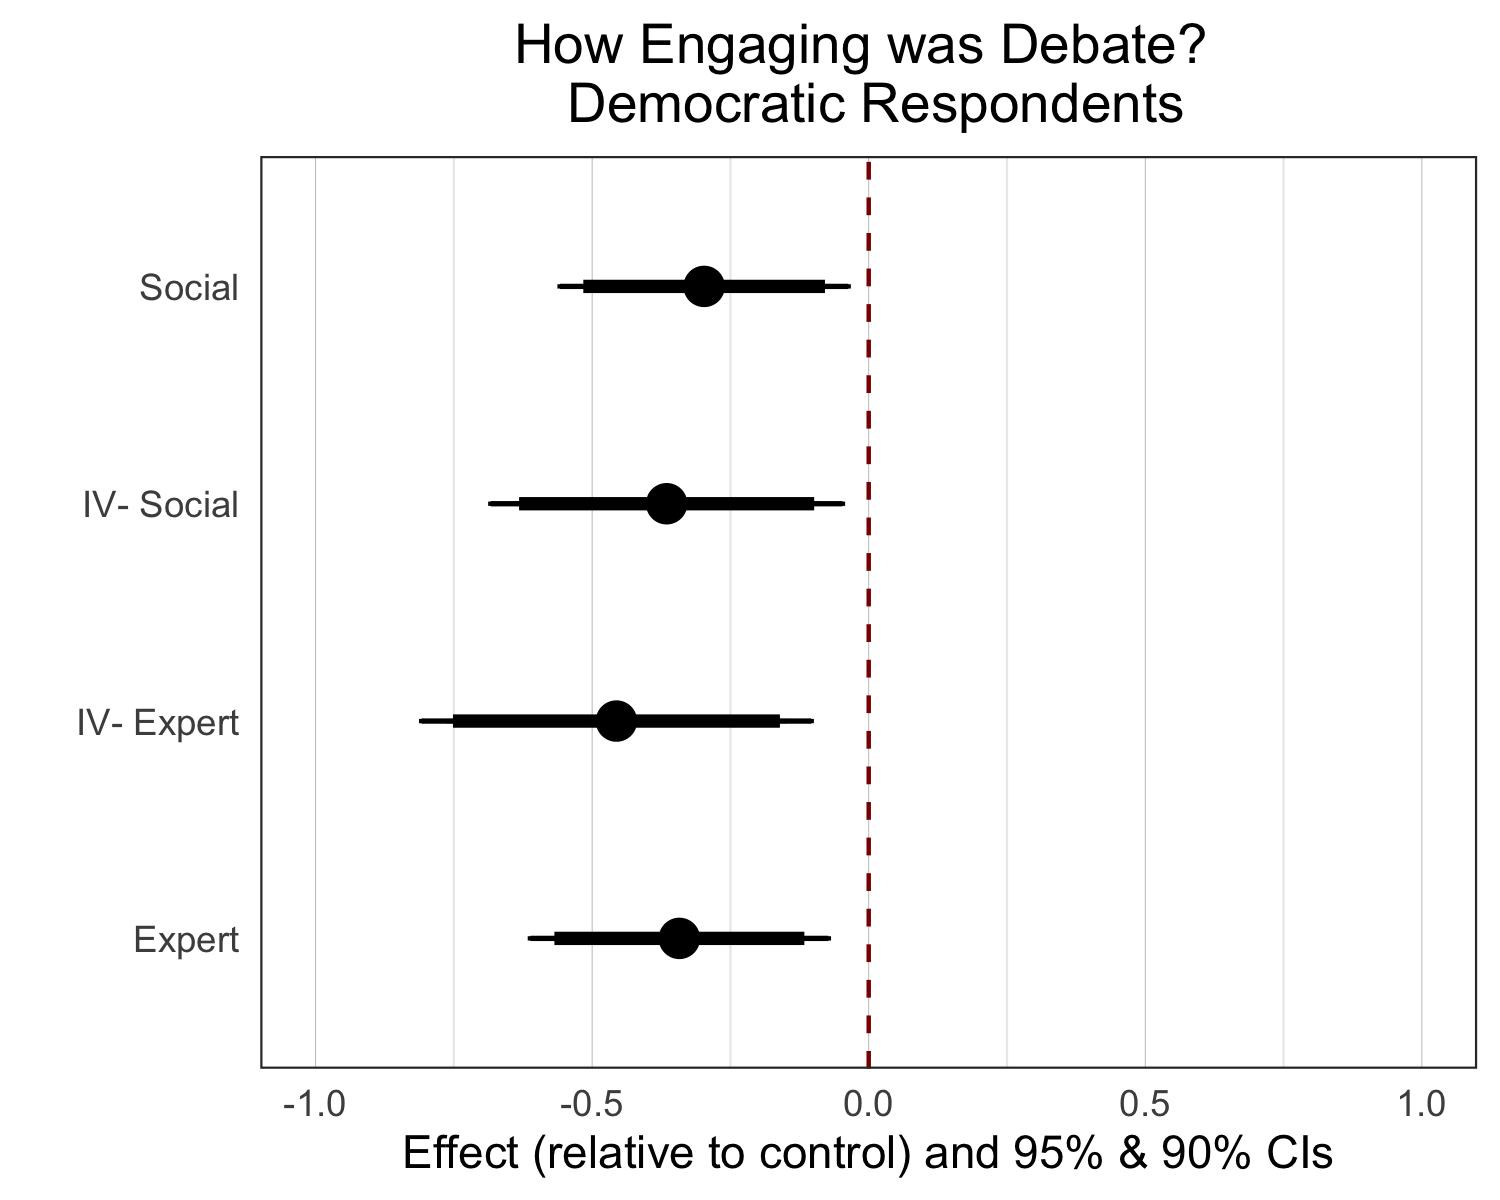
\includegraphics[width=.8\linewidth]{engaging_dem.png}

\end{frame}



\begin{frame}
\frametitle{Content Hypothesis Key Results}
Negative social chat associated with reduced candidate evaluation.
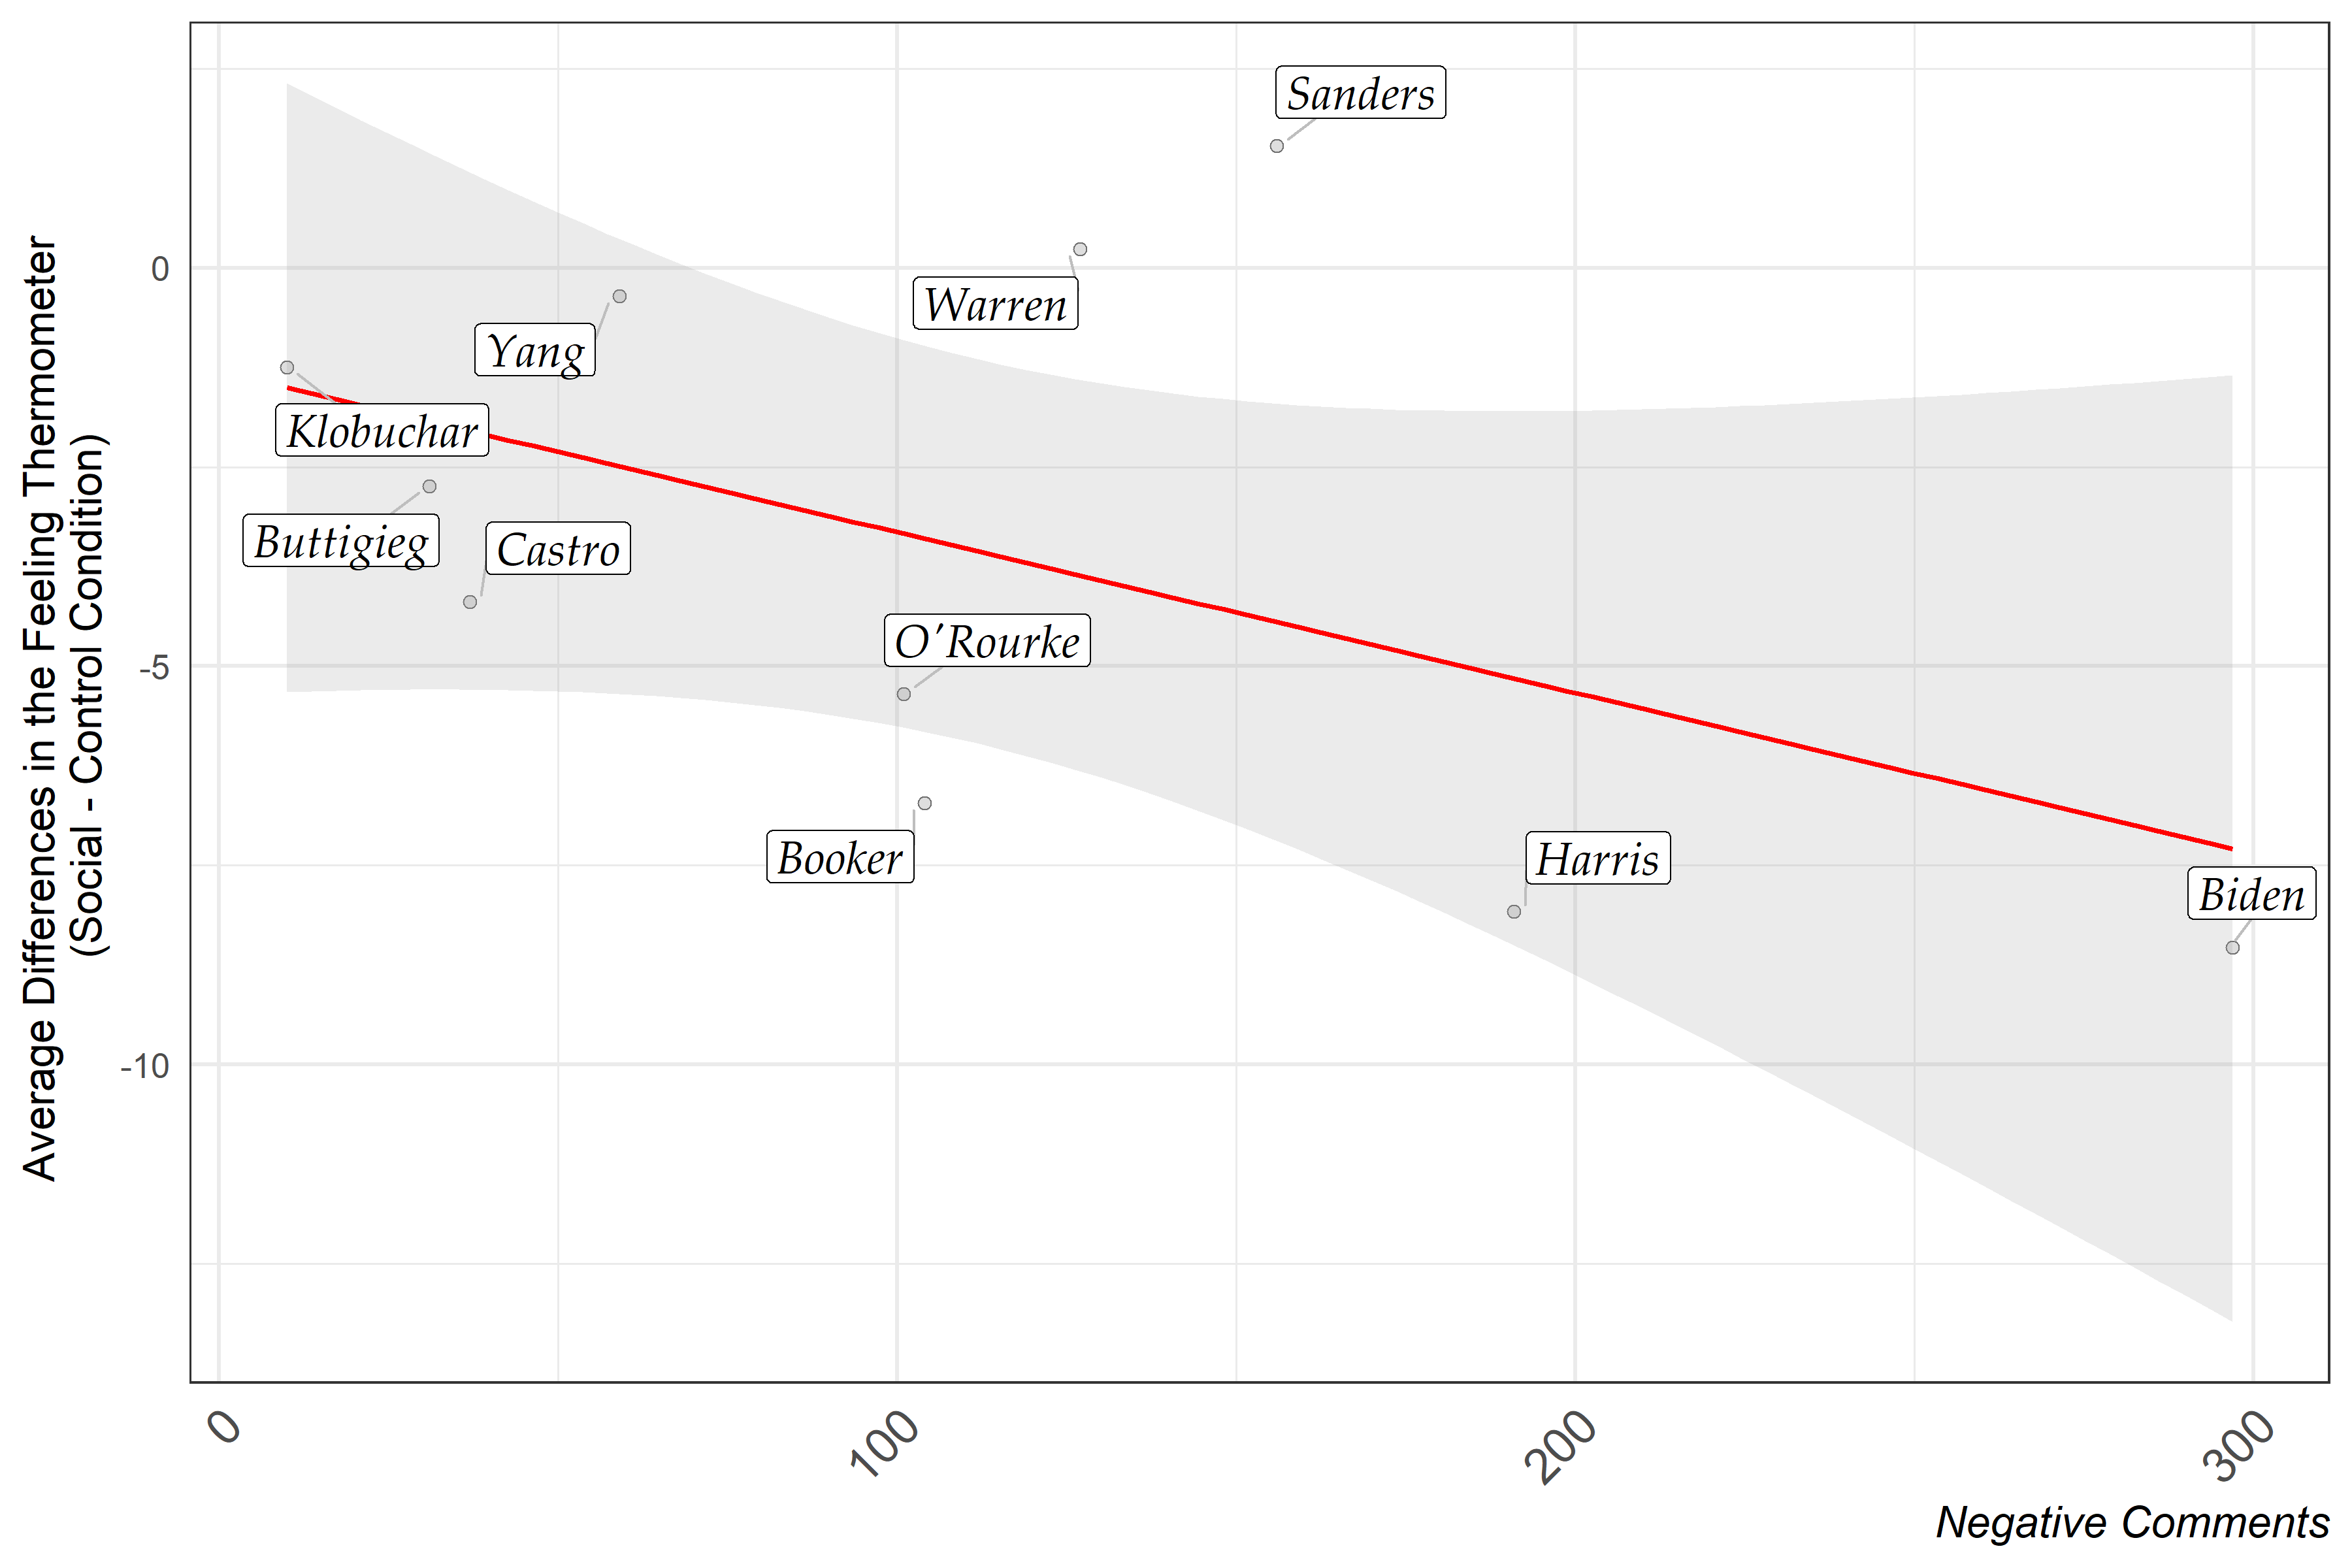
\includegraphics[width=.8\linewidth]{ft_on_negative_comments.png}
\end{frame}

\begin{frame}
\frametitle{Context Hypothesis Key Results}
Positive social chat associated with projected poll performance.
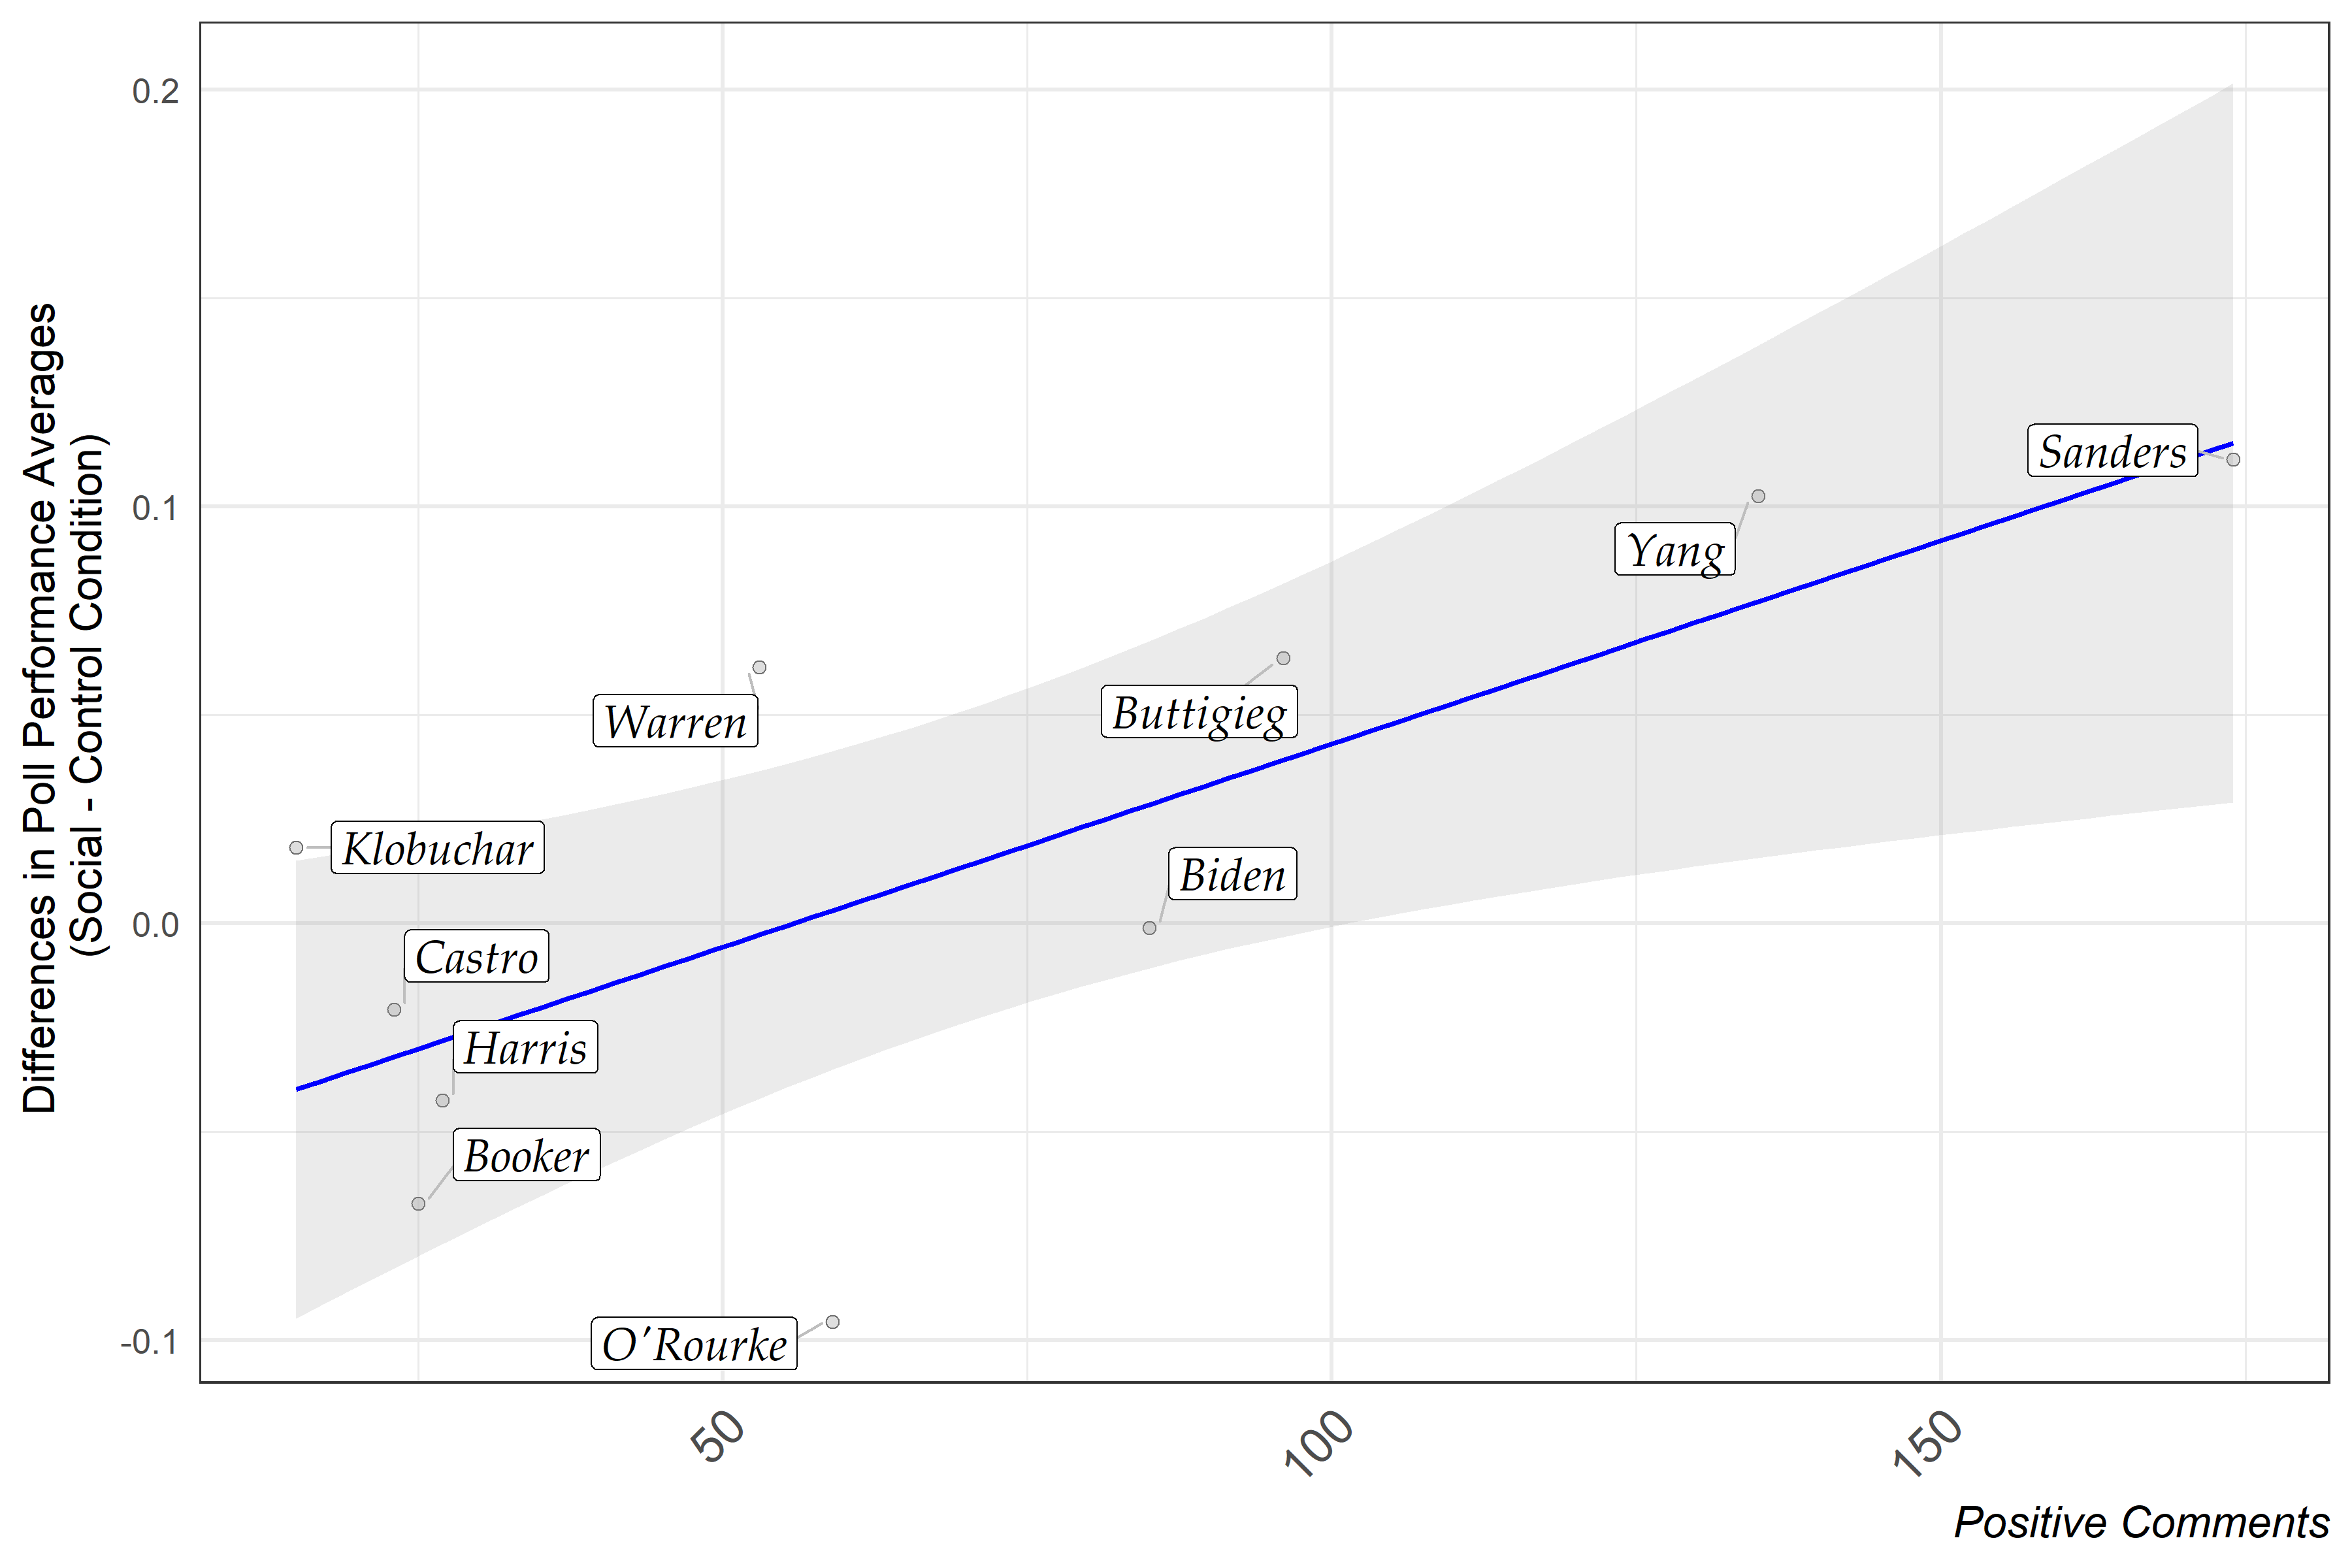
\includegraphics[width=.8\linewidth]{polls_on_positive_comments.png}
\end{frame}



\begin{frame}
\frametitle{Summary}

Streaming social chat 
\begin{itemize}
    \item Includes more frequent and more negative comments than expert chat.
\end{itemize}

\vspace{5mm}
\begin{itemize}
    \item Creates worse viewing experience.
    \item May disproportionately negatively affect certain candidates subject to toxic, negative comments.
    \item May distort inferences about candidate viability.
\end{itemize}

\vspace{5mm}
\begin{itemize}
    \item Less impact on overall trust and polarization.
    \item Less impact on name recognition.
\end{itemize}

\end{frame}

\begin{frame}
\frametitle{Implications and Next Steps}

Dual screening structurally alters study of media effects.
\begin{itemize}
    \item We identify three key dimensions: frequency, context, content.
\end{itemize}

\vspace{3mm}
Our findings give pause to use of streaming chat in politics.
\begin{itemize}
    \item Additional stimuli create potential for more interactivity.
    \item But come at a cost in terms of quality of viewing experience and inferences gained.
\end{itemize}


\vspace{3mm}
Next steps
\begin{itemize}
    \item Test hypotheses in new electoral contexts.
    \item Test mechanisms in laboratory setting with tighter control over compliance.
\end{itemize}



\end{frame}

\end{document}


